% Variational quantum metrology of notebook 44b, Eq. (1), drawn for N = 4.
% 1 prepare: hardware-efficient ansatz U(phi) on |0...0>;  2 noise: the same single-qubit channel E on every qubit;
% 3 encode: U_theta = exp(-i theta J_z) = prod_q R_z(theta);  4 measure: readout circuit V(phi'), then the computational basis.
% Optimisation 1 (Sections 5-7): maximise F = F_Q[sigma(phi), J_z], Eq. (2), over phi with the gradient of Eq. (12).
% Optimisation 2 (Section 8): maximise the classical Fisher information F_C, Eq. (14), over the readout angles.
\documentclass[tikz,border=6pt]{standalone}
\usepackage{amsmath,amssymb,bm}
\usetikzlibrary{arrows.meta,decorations.pathreplacing,calc,positioning}
\newcommand{\ket}[1]{\lvert #1\rangle}
\begin{document}
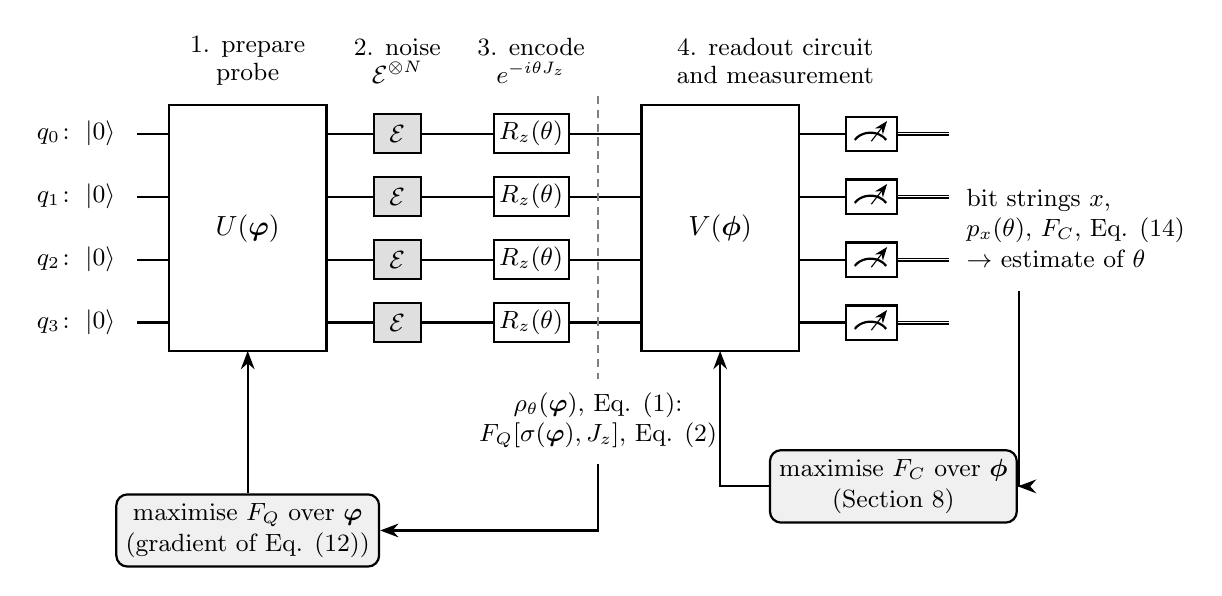
\begin{tikzpicture}[thick, >=Stealth, x=1cm, y=0.8cm,
    gate/.style={draw, fill=white, minimum height=0.5cm, minimum width=0.75cm, inner sep=2pt, font=\small},
    noise/.style={draw, fill=gray!25, minimum height=0.5cm, minimum width=0.6cm, inner sep=2pt, font=\small}]
  \foreach \q in {0,...,3} {
    \node[anchor=east, font=\small] at (-0.15,-\q) {$q_{\q}\!:\ \ket{0}$};
    \draw (0,-\q) -- (9.0,-\q); \draw[double, thin] (9.65,-\q) -- (10.3,-\q);
  }
  % 1 prepare
  \draw[fill=white] (0.4,0.45) rectangle (2.4,-3.45);
  \node at (1.4,-1.5) {$U(\boldsymbol\varphi)$};
  \node[font=\small, align=center] at (1.4,1.15) {1. prepare\\[-1pt] probe};
  % 2 noise
  \foreach \q in {0,...,3} \node[noise] at (3.3,-\q) {$\mathcal E$};
  \node[font=\small, align=center] at (3.3,1.15) {2. noise\\[-1pt] $\mathcal E^{\otimes N}$};
  % 3 encode
  \foreach \q in {0,...,3} \node[gate] at (5.0,-\q) {$R_z(\theta)$};
  \node[font=\small, align=center] at (5.0,1.15) {3. encode\\[-1pt] $e^{-i\theta J_z}$};
  % F_Q marker
  \draw[densely dashed, gray] (5.85,0.6) -- (5.85,-3.9);
  \node[font=\small, align=center, anchor=north] at (5.85,-3.95) {$\rho_\theta(\boldsymbol\varphi)$, Eq. (1):\\ $F_Q[\sigma(\boldsymbol\varphi),J_z]$, Eq. (2)};
  % 4 readout
  \draw[fill=white] (6.4,0.45) rectangle (8.4,-3.45);
  \node at (7.4,-1.5) {$V(\boldsymbol\phi)$};
  \foreach \q in {0,...,3} {
    \draw[fill=white] (9.0,-\q+0.27) rectangle (9.65,-\q-0.27);
    \draw (9.11,-\q-0.1) arc (150:30:0.23);
    \draw[->, thin] (9.32,-\q-0.12) -- (9.52,-\q+0.2);
  }
  \node[font=\small, align=center] at (8.1,1.15) {4. readout circuit\\[-1pt] and measurement};
  \node[font=\small, anchor=west, align=left] at (10.4,-1.5) {bit strings $x$,\\ $p_x(\theta)$, $F_C$, Eq. (14)\\ $\to$ estimate of $\theta$};
  % optimisation loops
  \node[draw, rounded corners, fill=gray!12, font=\small, align=center] (o1) at (1.4,-6.3)
       {maximise $F_Q$ over $\boldsymbol\varphi$\\ (gradient of Eq. (12))};
  \draw[->] (5.85,-5.25) |- (o1.east);
  \draw[->] (o1.north) -- (1.4,-3.45);
  \node[draw, rounded corners, fill=gray!12, font=\small, align=center] (o2) at (9.6,-5.6)
       {maximise $F_C$ over $\boldsymbol\phi$\\ (Section 8)};
  \draw[->] (11.2,-2.5) |- (o2.east);
  \draw[->] (o2.west) -| (7.4,-3.45);
\end{tikzpicture}
\end{document}
